\documentclass[conference]{IEEEtran}
\IEEEoverridecommandlockouts

\usepackage{amsmath,amssymb}
\usepackage{booktabs,multirow,colortbl}
\usepackage{graphicx}
\usepackage{xcolor}
\usepackage{pgfplots}
\pgfplotsset{compat=1.18}
\usepackage{siunitx}
\usepackage[hidelinks]{hyperref}
\usepackage[capitalise,nameinlink]{cleveref}
\usepackage{cite}

% placement colours, used consistently in every figure
\definecolor{cmag}{HTML}{1F6F8B}
\definecolor{cfis}{HTML}{6A8F3A}
\definecolor{cgrad}{HTML}{C0612B}
\definecolor{crand}{HTML}{8A939C}
\pgfplotsset{
  accplot/.style={width=\columnwidth,height=5.2cm,grid=major,grid style={gray!20},
    tick label style={font=\scriptsize},label style={font=\footnotesize},
    legend style={font=\scriptsize,draw=none,fill=white,fill opacity=0.85,text opacity=1},
    legend cell align=left,ylabel={SST-2 accuracy (\%)},ymin=45,ymax=93,mark size=1.2pt},
  pslc/.style={black,densely dotted,thick,mark=square*,mark options={solid}},
  pmlc/.style={black!55,dashdotted,thick,mark=triangle*,mark options={solid}},
  pmag/.style={cmag,very thick,mark=*},
  pfis/.style={cfis,thick,dashed,mark=diamond*,mark options={solid}},
  pgrad/.style={cgrad,thick,mark=*},
  prand/.style={crand,thick,mark=o}}


% float-only pages start at the top instead of being centred
\makeatletter\setlength{\@fptop}{0pt}\makeatother

\begin{document}

\title{Reliable Hybrid SLC/MLC ReRAM\\ Crossbars for Transformers\\[4pt]
{\Large Component Placement, Fault-Aware Mapping and Noise-Aware Training}}

\author{\IEEEauthorblockN{Shivansh Mittal\qquad Sarvesh Joshi\qquad Thumati Naveen Chandra Chowdary\qquad
Aryan Chakravorty}
\IEEEauthorblockA{\textit{Indian Institute of Technology Guwahati}\\
Course Project, CS5290 Memory-Centric Computer Architecture}}

\maketitle

\begin{abstract}
Hybrid ReRAM crossbars keep the most important weights in reliable single-level cells (SLC) and the rest
in dense multi-level cells (MLC). HyFlexPIM applies this to transformers by factorising each weight
matrix with SVD and protecting the components with the largest loss gradients. We evaluate this scheme on
BERT-Base and DistilBERT (SST-2) with a bit-accurate crossbar simulator that models errors cell by cell:
programming and read noise, level-dependent noise, stuck cells, a fixed ADC with bit-serial inputs and IR
drop. A hybrid layout is necessary, since all-MLC storage falls to 52--60\% accuracy at 7.5\% programming noise,
but the choice of components matters as much as their number. Ranking components by singular value
reaches the same accuracy as a Fisher-information estimate of each component's expected damage, while a
gradient score loses 2--12 points at high noise; we explain this through the per-column quantisation of the
crossbar. With magnitude ranking, 5--10\% of components in SLC match an all-SLC chip at 5\% noise.
Stuck cells are the one effect placement cannot handle. Because the components of an SVD layer can be
stored in any order, we map them to physical slots around a tested chip's stuck cells by solving an
assignment problem, at no hardware cost; this raises BERT-Base at 0.5\% stuck cells from 76.6\% to
85.6\%. Fine-tuning on simulated chips with stuck cells adds to this mapping. A tier-aware variant, which
trains each component under the errors of the tier (SLC or MLC) it will be stored in, lifts BERT-Base at 1\% stuck cells from 65.1\% to 82.9\%,
so that the hybrid chip matches or exceeds an all-SLC chip with mapping up to 1\% scattered stuck cells,
using 34\% fewer cells. The placement and mapping results also hold
on MNLI.
\end{abstract}

\begin{IEEEkeywords}
ReRAM, processing-in-memory, multi-level cell, stuck-at faults, SVD, transformer, fault-aware mapping, noise-aware training
\end{IEEEkeywords}

\section{Introduction}\label{sec:intro}

\IEEEPARstart{R}{esistive} RAM (ReRAM) crossbars compute a matrix--vector product where the weights are
stored. Each weight is held as the conductance of one or more resistive cells; applying the input as
row voltages makes each column current the dot product of the input with that column's
conductances~\cite{shafiee2016isaac,chi2016prime}. Weights never move between memory and compute, which
removes most of the data movement that dominates the energy of neural-network inference on conventional
hardware. The cost is accuracy: a cell cannot be programmed to an exact conductance, its reading
fluctuates, and some cells are permanently stuck at their highest or lowest conductance.

A cell can store one bit (single-level cell, SLC) or several bits (multi-level cell, MLC). MLC is denser,
but its conductance levels are closer together, so the same conductance error corrupts more of the stored
value. HyFlexPIM~\cite{song2025hyflexpim} combines the two for transformers: it factorises each weight
matrix with singular value decomposition (SVD), keeps the components with the largest loss gradients in
SLC and stores the rest in MLC (\cref{sec:background}). Its evaluation applies relative noise to whole
weights at a single noise level.

We revisit this design with errors modelled cell by cell, as they arise in hardware, and ask which
components should be protected, how many, and which hardware effects still break the scheme. We study
BERT-Base~\cite{devlin2019bert} and DistilBERT~\cite{sanh2019distilbert} on the SST-2 sentiment
task~\cite{socher2013sst,wang2019glue}, and repeat the placement and mapping study on MNLI.

\textbf{Our contributions.} We keep HyFlexPIM's SVD factorisation and hybrid layout unchanged and add the
following.
\begin{itemize}
\item \textbf{Cell-level evaluation} (\cref{sec:model}). HyFlexPIM perturbs whole weights at one noise
level. We build a verified crossbar model that adds noise to every cell of a differential pair and its bit
slices, sweep programming noise from 0 to 10\%, and add read noise, level-dependent MLC noise, three
patterns of stuck cells, a fixed ADC with bit-serial inputs and IR drop. Every configuration is compared
on the same simulated chips.

\item \textbf{Which components to protect, and why} (\cref{sec:placement,sec:discussion}). HyFlexPIM ranks
components by their loss gradient. We show that ranking by singular value is as good as a
Fisher-information estimate of each component's expected damage and better than the gradient at high
noise, and explain this through the per-column quantisation of the crossbar.

\item \textbf{Stuck cells as the limiting effect.} HyFlexPIM does not model stuck cells. We find that every
other effect leaves the magnitude hybrid within about a point of all-SLC, while stuck cells break every
placement.

\item \textbf{Fault-aware mapping for SVD layers} (\cref{sec:mapping}). The components of an SVD layer can
be stored in any order. We use this freedom to place components around a tested chip's stuck cells, by a
Fisher-weighted assignment of components to slots, with no extra hardware or retraining.

\item \textbf{Tier-aware training} (\cref{sec:training}). In HyFlexPIM, hardware noise is applied only at
inference, not during fine-tuning. We train on simulated chips, with each component under the errors of the tier (SLC or MLC) it
will be stored in. Together with mapping, this lets the hybrid chip match an all-SLC chip with mapping up
to 1\% scattered stuck cells, using 34\% fewer cells.
\end{itemize}

\Cref{sec:background} reviews background and related work, \cref{sec:model,sec:placement,%
sec:mapping,sec:training} describe the model and methods, \cref{sec:setup,sec:results,sec:mnli} the experiments,
and \cref{sec:discussion,sec:conclusion} discuss and conclude.

\section{Background and Related Work}\label{sec:background}

\subsection{Matrix--Vector Products in a ReRAM Crossbar}
A crossbar places a resistive cell at every crossing of a row (word line) and a column (bit line). If
cell $(i,j)$ has conductance $G_{ij}$ and row $i$ is driven at voltage $V_i$, the current collected at
column $j$ is
\begin{equation}
I_j=\sum_i V_i\,G_{ij},
\label{eq:crossbar}
\end{equation}
by Ohm's law in each cell and Kirchhoff's current law on the column. One read therefore computes a full
matrix--vector product in the analog domain. Accelerators such as ISAAC~\cite{shafiee2016isaac} and
PRIME~\cite{chi2016prime} build on this primitive. Three conventions from these designs are used
throughout this report:
\begin{itemize}
\item Conductances are non-negative, so a signed weight is stored as the difference of two cells, a
\emph{differential pair}.
\item A cell holds only a few bits, so a multi-bit weight is split into \emph{bit slices} on separate
cells; the column results of the slices are shifted and added digitally.
\item Arrays have a fixed size (we use $128\times128$ tiles), and an analog-to-digital converter (ADC)
digitises each column current.
\end{itemize}

\subsection{SLC, MLC and Non-Idealities}
A cell programmed to $L=2^b$ levels between $G_{\min}$ and $G_{\max}$ stores $b$ bits; $b=1$ is a
single-level cell (SLC) and $b\geq2$ a multi-level cell (MLC). The level spacing is
$\Delta=(G_{\max}-G_{\min})/(L-1)$, so a two-bit cell has levels three times closer than an SLC. A
conductance error of fixed size is therefore three times larger relative to an MLC level, while MLC
needs fewer cells per weight. Real arrays deviate from the programmed state in several ways:
\begin{itemize}
\item \emph{Programming variation}: each cell lands near, not on, its target conductance; the error is
fixed once the chip is programmed.
\item \emph{Read noise}: the current fluctuates at every read.
\item \emph{Stuck-at faults}: some cells are permanently stuck at $G_{\max}$ or $G_{\min}$, whatever
is written; faults can be scattered, clustered, or affect a whole line.
\item \emph{IR drop}: wire resistance lowers the voltage reaching cells far from the drivers.
\item \emph{ADC resolution}: column currents are rounded to a limited number of levels.
\end{itemize}

\subsection{HyFlexPIM}
HyFlexPIM~\cite{song2025hyflexpim} is a mixed-signal processing-in-memory accelerator for
transformers. Its analog part can switch each array between SLC and MLC operation, so that critical
weights use SLC and the rest use denser, cheaper MLC. Placing raw weights this way gives little benefit,
because importance is spread over many weights. HyFlexPIM therefore factorises each weight matrix with a
truncated SVD, $W\approx U\Sigma V^{\top}$, and fine-tunes the factors, which concentrates the loss
gradient in a small subset of components; it calls this \emph{gradient redistribution}. Components are
ranked by the gradient of the loss with respect to their singular value, and the top-ranked share is
mapped to SLC. Accuracy is evaluated with relative Gaussian noise applied to whole weights,
$\tilde W=W\odot(1+\eta)$, at a single level derived from a measured MLC bit error
rate~\cite{fan2024mlc}, together with a limited ADC resolution. Stuck cells, read noise and IR drop are
not modelled. Our work keeps the SVD
factorisation and the hybrid layout unchanged; \cref{sec:intro} lists what it adds.

\subsection{Fault-Tolerant Mapping and Training}
Two families of methods make crossbar inference tolerant to device errors. The first adapts training to
the hardware. Chen \emph{et al.}~\cite{chen2017accelerator} include device variations and defects in
training. Xia \emph{et al.}~\cite{xia2017fault} detect stuck cells on line and adapt training to them.
Rasch \emph{et al.}~\cite{rasch2023hwa} inject hardware noise during training at scale, in what is now
called hardware-aware training; gradients pass through the non-differentiable hardware model with a
straight-through estimator~\cite{bengio2013ste}. The second family leaves the weights unchanged and
chooses \emph{where} they are stored, so that important values avoid faulty cells. Such mapping
problems reduce to assignment problems, which the Hungarian method~\cite{kuhn1955hungarian} solves
exactly.

Our fault-aware mapping belongs to the second family, with two differences. First, the freedom to
reorder comes from the SVD itself: the components of a factorised layer can be stored in any order
without changing its output, so no permutation hardware or change to neighbouring layers is needed.
Second, the cost of a placement is weighted by the Fisher information of each stored value, a
second-order estimate of loss sensitivity in the spirit of Optimal Brain
Damage~\cite{lecun1990obd} and of Fisher-based importance in continual
learning~\cite{kirkpatrick2017ewc}.

\section{Crossbar Model}\label{sec:model}

We wrote a PyTorch simulator that replaces each linear layer of a model with crossbars and models the
stored value of every cell. This section describes how a weight matrix is stored, the error sources,
and how the simulator was verified. \Cref{tab:model} lists the parameters.

\begin{table}[t]
\centering\footnotesize
\caption{Crossbar model parameters.}\label{tab:model}
\setlength{\tabcolsep}{4pt}
\begin{tabular}{@{}ll@{}}
\toprule
Parameter & Value \\
\midrule
Weight precision & 8-bit signed, one scale per output column \\
Input precision & 8-bit signed \\
Cells per weight (per sign) & 7 SLC ($b=1$) or 4 MLC ($b=2$) \\
Conductance range & $G_{\max}=1$ (normalised), $G_{\max}/G_{\min}=100$ \\
Tile size & $128\times128$ \\
Programming noise $\sigma$ & 0--10\% of $G_{\max}$, fixed per chip \\
Read noise $\sigma_r$ & 0.5--5\% of $G_{\max}$, fresh at every read \\
Stuck cells $p$ & 0.1--5\% of cells, half at $G_{\max}$, half at $G_{\min}$ \\
ADC & ideal, or 3--8 bits with a fixed calibrated range \\
Wire resistance $r$ & $R_{\text{wire}}$ per segment / $R_{\text{on}}$, $10^{-4}$--$3\times10^{-3}$ \\
\bottomrule
\end{tabular}
\end{table}

\subsection{Storing a Weight Matrix}
A matrix $W\in\mathbb R^{m\times n}$, with $n$ inputs and $m$ outputs, is stored with its inputs on the rows
(word lines) and its outputs on the columns (bit lines) of the crossbar. It is quantised to signed 8-bit
integers with one scale per output column,
\begin{equation}
q_{ij}=\operatorname{clip}\!\big(\operatorname{round}(w_{ij}/s_i),\,-127,\,127\big),
\label{eq:quant}
\end{equation}
with column scale $s_i=\max_j|w_{ij}|/127$ for output $i$.
The sign is handled by a differential pair, $q=q^{+}-q^{-}$ with $q^{\pm}=\max(\pm q,0)$, and each
7-bit magnitude is split into $S=\lceil 7/b\rceil$ base-$L$ digits,
\begin{equation}
q^{\pm}=\sum_{t=0}^{S-1}L^{t}d_t^{\pm},\qquad d_t^{\pm}\in\{0,\dots,L-1\},
\label{eq:slice}
\end{equation}
each stored in its own cell at conductance $G=G_{\min}+d\,\Delta$. An SLC weight thus uses $2\times7$
cells and an MLC weight $2\times4$. The stored weight is read back as
\begin{equation}
\hat w_{ij}=s_i\sum_{t=0}^{S-1}L^{t}\,\frac{G^{+}_{ij,t}-G^{-}_{ij,t}}{\Delta},
\label{eq:readback}
\end{equation}
where the $G_{\min}$ offset cancels in the difference. Without errors, $\hat w_{ij}=s_iq_{ij}$ exactly.
Inputs are quantised to 8 bits in the same way with one scale per tensor, and the layer output is the
product of the quantised input with $\hat W$.

\subsection{Error Sources}
Each error source is a separate, seeded option, so that its effect can be measured on its own.
\begin{itemize}
\item \textbf{Programming noise.} Every cell receives a fixed Gaussian offset,
$\tilde G=\max\!\big(0,\;G+\sigma G_{\max}\varepsilon\big)$ with $\varepsilon\sim\mathcal N(0,1)$, drawn
once per chip. Because $\Delta$ is three times smaller for MLC, the same $\sigma$ causes a three times
larger digit error in MLC.

\item \textbf{Level-dependent noise.} The noise of an MLC cell can depend on its level: $\sigma$ is
multiplied by a factor $m_d$ per level $d$. We use $m=(1,1.5,1.5,1)$ and $m=(1,2,2,1)$, making the two
middle levels up to twice as noisy as the end levels.

\item \textbf{Read noise.} An independent Gaussian offset of standard deviation $\sigma_r G_{\max}$ is
added to every cell at every read. Since it is independent of the stored value, its effect on an output
is Gaussian with a closed-form variance, which the simulator adds directly to the output.

\item \textbf{Stuck cells.} A cell is stuck with probability $p$, at $G_{\max}$ or $G_{\min}$ with equal
probability, and keeps that conductance whatever is written. In the \emph{clustered} pattern, faults
grow from random seeds into $3\times3$ blocks, with the seed rate set so that the overall rate is about
$p$. In the \emph{line} pattern, a whole bit line within one $128$-row tile fails with probability $p$.

\item \textbf{ADC and bit-serial inputs.} With a finite ADC, inputs are applied one bit at a time:
each input is written in sign-magnitude form, and bit $k$ of its magnitude is applied with the input's
sign. For every input bit $k$, weight slice $t$ and $128$-row tile, the column sum is quantised by a
$b_{\text{ADC}}$-bit ADC and the results are combined digitally,
\begin{equation}
y_j=\sum_{k}\sum_{t}2^{k}L^{t}\,\mathrm{ADC}_t\!\Big(\sum_{i\in\text{tile}}x_i^{(k)}\big(d^{+}_{ij,t}-d^{-}_{ij,t}\big)\Big).
\label{eq:adc}
\end{equation}
The full-scale range of each slice's ADC is fixed once, from the largest column sum observed on 64
training sentences on an error-free chip, and is not adjusted at run time.

\item \textbf{IR drop.} A first-order static model attenuates each cell by its distance from the row
driver and the column sense amplifier. A cell crossed by $n$ wire segments behaves as
\begin{equation}
G_{\text{eff}}=\frac{G}{1+r\,G\,n},\qquad n=(c+1)+(127-\rho),
\label{eq:irdrop}
\end{equation}
where $c$ and $\rho$ are the cell's column and row positions within its tile, and $r$ is the resistance
of one wire segment relative to the on-resistance. This ignores the dependence of IR drop on the input
pattern, which is enough to show whether a cell's position matters.
\end{itemize}

\subsection{Chips and Paired Comparison}
A \emph{chip} is one draw of all random errors in a model: noise offsets, stuck cells and their values.
All draws come from a single random generator seeded with the chip number, and every placement or
mapping is evaluated on the same seeds. Two placements are therefore compared on chips with identical
error draws, and their difference on each chip is a paired measurement. We report the mean accuracy
over chips and, where differences are small, the mean paired difference with its standard error.

\subsection{Verification}
Every experiment starts with self-tests on random matrices, and stops if any check fails:
\begin{itemize}
\item With all errors disabled, the crossbar output equals the 8-bit integer product to a relative
error below $10^{-4}$, for SLC and MLC, both in one pass and when read slice by slice, tile by tile and
bit by bit.
\item The bit planes of an input rebuild it exactly.
\item A calibrated 16-bit ADC is lossless to a relative error below $10^{-3}$, while a 4-bit ADC is not.
\item The measured spread of read noise matches its closed-form variance to within 15\%.
\item The three fault patterns produce the requested share of stuck cells.
\item IR drop only reduces stored conductances, and level-dependent noise with all factors equal to one
reproduces plain programming noise exactly.
\end{itemize}
End to end, a chip with no errors reaches within about one point of the digital model for every placement
(\cref{sec:results}).

\section{SVD Tiering and Component Placement}\label{sec:placement}

\subsection{Factorisation and Fine-Tuning}
Following HyFlexPIM~\cite{song2025hyflexpim}, every linear layer of the transformer encoders (72
matrices in BERT-Base, 36 in DistilBERT) is factorised with a truncated SVD,
\begin{equation}
W\approx U\Sigma V^{\top}=\sum_{r=1}^{k}\sigma_r\,u_r v_r^{\top},\qquad
k=\Big\lfloor\frac{mn}{m+n}\Big\rfloor,
\label{eq:svd}
\end{equation}
for $W\in\mathbb R^{m\times n}$. This rank keeps the parameter count unchanged, e.g.\ $k=384$ for a
$768\times768$ attention matrix and $k=614$ for a $768\times3072$ feed-forward matrix. Truncation loses
accuracy, so the factorised model is fine-tuned on the full SST-2 training set (67{,}349 sentences) for 8
epochs with AdamW, learning rate $2\times10^{-5}$ with linear decay, and batch size 32. $U$, $\Sigma$ and
$V$ are trained directly, so the factors need not stay orthogonal.

\subsection{Mapping a Factorised Layer onto Two Tiers}
We call $(\sigma_r,u_r,v_r)$ the $r$-th \emph{component}. On the chip it is stored as one column of a first
crossbar, holding $\sigma_r v_r$, and one row of a second crossbar, holding $u_r$: the first crossbar turns
the input into one value per component, and the second spreads each value back over the outputs. A placement chooses a set
$\mathcal S$ of components for SLC; the rest form the MLC tier. Each tier has its own pair of crossbars
(\cref{fig:tiers}), and the layer computes
\begin{equation}
y=U_{\mathcal S}\big(\Sigma V^{\top}\big)_{\mathcal S}\,x+U_{\bar{\mathcal S}}\big(\Sigma V^{\top}\big)_{\bar{\mathcal S}}\,x+b.
\label{eq:tiers}
\end{equation}
The intermediate vector between the two crossbars is re-quantised to 8 bits, as any crossbar input. A
component holds $m+n$ weights, so placing a share $f$ of the components in SLC costs $14f+8(1-f)$ cells per
weight against 14 for all-SLC; at $f=20\%$ this is 9.2 cells, 34\% fewer. All placements select the top
$\lceil fk\rceil$ components of each layer by a score, so every layer has the same SLC share.

\begin{figure}[t]
\centering
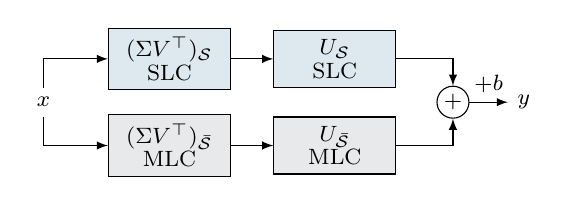
\begin{tikzpicture}[font=\footnotesize,
  xb/.style={draw,minimum width=1.55cm,minimum height=0.62cm,align=center},
  arr/.style={-latex}]
\node (x) at (0,0) {$x$};
\node[xb,fill=cmag!15] (s1) at (1.6,0.55) {$(\Sigma V^{\top})_{\mathcal S}$\\[-1pt]SLC};
\node[xb,fill=cmag!15] (s2) at (3.7,0.55) {$U_{\mathcal S}$\\[-1pt]SLC};
\node[xb,fill=crand!20] (m1) at (1.6,-0.55) {$(\Sigma V^{\top})_{\bar{\mathcal S}}$\\[-1pt]MLC};
\node[xb,fill=crand!20] (m2) at (3.7,-0.55) {$U_{\bar{\mathcal S}}$\\[-1pt]MLC};
\node[draw,circle,inner sep=1pt] (p) at (5.2,0) {$+$};
\node (y) at (6.1,0) {$y$};
\draw[arr] (x) |- (s1); \draw[arr] (x) |- (m1);
\draw[arr] (s1) -- (s2); \draw[arr] (m1) -- (m2);
\draw[arr] (s2) -| (p); \draw[arr] (m2) -| (p);
\draw[arr] (p) -- node[above] {$+b$} (y);
\end{tikzpicture}
\caption{A factorised layer on the chip. Components in $\mathcal S$ use SLC crossbars, the rest MLC
crossbars; each component is one column of the first crossbar and one row of the second.}
\label{fig:tiers}
\end{figure}

\subsection{Placement Scores}
Besides the two extremes, all-SLC and all-MLC, and a random choice as a control, we compare three scores.
All data-dependent scores use the same 2{,}048 SST-2 training sentences.

\textbf{Magnitude.} The size of the singular value, $|\sigma_r|$ ($\sigma_r$ is trained freely and need
not stay positive). It needs no data.

\textbf{Gradient (HyFlexPIM-style).} The absolute loss gradient with respect to the singular value,
summed over batches $b$ of 32 sentences with dropout active,
\begin{equation}
g_r=\sum_b\Big|\frac{\partial L_b}{\partial\sigma_r}\Big|.
\label{eq:grad}
\end{equation}
The absolute value is taken per batch because, on a trained model, the gradients of different sentences
point in opposite directions and largely cancel in a single sum.

\textbf{Fisher.} The expected rise in loss if component $r$ is stored in MLC. To second order, a small
random error $\delta_e$ on stored entry $e$ raises the expected loss by about $\tfrac12F_e\,\mathbb
E[\delta_e^2]$, where $F_e$ is the Fisher information of that entry~\cite{lecun1990obd}. We estimate $F_e$
by the empirical Fisher, the sum of squared per-sentence gradients. Under the cell model of
\cref{sec:model}, a fixed cell noise becomes a weight error proportional to the 8-bit scale of the
crossbar column holding the entry, so $\mathbb E[\delta_e^2]\propto s^2$. Summing over every entry the
component stores gives
\begin{equation}
D_r=s_r^2\sum_j F\big(\sigma_r v_{rj}\big)+\sum_i t_i^2\,F\big(u_{ir}\big),
\label{eq:fisher}
\end{equation}
where $s_r=\max_j|\sigma_r v_{rj}|/127$ is the scale of the component's column in the first crossbar and
$t_i=\max_r|u_{ir}|/127$ that of output column $i$ in the second. The constant factor of the noise variance
is the same for every component and is omitted.

\section{Fault-Aware Mapping}\label{sec:mapping}

Placement decides which tier each component uses, but not which physical row of that tier. With stuck
cells this matters: a stuck high-order cell shifts its weight by a large fixed amount, so it does far
more harm under an important component than under an unimportant one. This section uses a property of
the SVD layer to choose the row of every component around a chip's stuck cells.

\subsection{Free Order of Components}
For any permutation matrix $P$,
\begin{equation}
(UP)\big(P^{\top}\Sigma V^{\top}\big)=U\Sigma V^{\top},
\label{eq:perm}
\end{equation}
so the $k$ components of a layer can be stored in any order without changing its output. We call the
$j$-th position of a tier a \emph{slot}: row $j$ of the tier's first crossbar together with column $j$ of
its second crossbar. Moving a component to another slot moves its row $\sigma_r v_r^{\top}$ and its
column $u_r$ together. The order is fixed when the chip is programmed, so a chosen mapping needs no
permutation hardware and no change to the neighbouring layers.

\subsection{Known Stuck Cells}
Stuck cells can be located after fabrication by writing and reading back every cell. We assume this test
has been done, so each chip's stuck-cell map is known before its weights are programmed; in simulation it
is the chip's drawn fault map. Programming noise is random and not known in advance, so the mapping
targets stuck cells only.

\subsection{Cost of a Component in a Slot}
Placing component $r$ in slot $s$ costs the expected rise in loss caused by the stuck cells of that slot.
A cell of slice $t$ stuck at conductance $G^{*}$, under an entry whose digit should be $d$, changes the
entry by
\begin{equation}
\delta=\pm\,s\,L^{t}\,\frac{G^{*}-(G_{\min}+d\,\Delta)}{\Delta},
\label{eq:stuckerr}
\end{equation}
with $s$ the 8-bit scale of the crossbar row holding the entry and the sign set by the side of the
differential pair. Weighting each error by the Fisher information of its entry, as in \cref{eq:fisher},
gives
\begin{equation}
C_{rs}=\sum_{\text{stuck cells }c\text{ in slot }s}F_{e(r,c)}\,\delta_{r,c}^{2},
\label{eq:cost}
\end{equation}
where $e(r,c)$ is the entry of component $r$ that would occupy cell $c$. The first-crossbar row moves with
its component and keeps its own scale $s_r$, while the scales $t_i$ of the second crossbar depend only on
which components share the tier, so every term of $C_{rs}$ is known before programming. The sum treats two
stuck cells under the same entry as independent, which slightly misestimates their joint error; it is
exact when each entry has at most one stuck cell.

\subsection{Assignment}
Within each tier, the mapping is the permutation $\pi$ that minimises $\sum_r C_{r\pi(r)}$, a linear
assignment problem. We solve it exactly with the Hungarian method~\cite{kuhn1955hungarian} as implemented
in SciPy~\cite{virtanen2020scipy}, separately for every layer and tier; cost matrices have at most
$614\times614$ entries (all components of a feed-forward layer). We apply it to the
magnitude hybrid, keeping its SLC set and choosing the slot of each component within its tier; this is
our \emph{fault-aware mapping}. As a high-cost reference, we apply the same mapping to an all-SLC chip.

\subsection{Joint Tier and Slot Mapping}
Fault-aware mapping keeps the SLC set fixed. A natural extension chooses tier and slot together for each
chip: an important component might be better off in a clean MLC slot than in a badly damaged SLC slot. We
form one assignment over all $k$ components and all $k$ slots of a layer, with $\lceil fk\rceil$ SLC slots,
which enforces the SLC budget. The cost of a slot adds the expected damage from programming noise in its
tier to \cref{eq:cost},
\begin{equation}
C^{\text{joint}}_{rs}=C_{rs}+\kappa_{\tau(s)}\Big(s_r^2\sum_j F\big(\sigma_r v_{rj}\big)+\sum_i t_i^2F\big(u_{ir}\big)\Big),
\label{eq:c1}
\end{equation}
where $\kappa_\tau=2(\sigma_d/\Delta_\tau)^2\sum_t L_\tau^{2t}$ is the noise variance of a weight in tier
$\tau$, in units of its 8-bit step. The second term is the Fisher score $D_r$ of \cref{eq:fisher} scaled
by the tier. We use $\sigma_d=\max(\sigma,2\%)$, so that on a chip with stuck cells but no programming noise
the tier choice still reflects the higher fragility of MLC.

\subsection{Checking the Cost Model}
Before every run, a self-test programs a random layer with a known fault map and compares the predicted
cost $\sum_r C_{rr}$ with the actual Fisher-weighted error of the programmed crossbar. The run stops unless
the two agree to within 10\% for both SLC and MLC, and unless the assignment does not increase the cost.

\section{Noise- and Fault-Aware Training}\label{sec:training}

Mapping leaves the weights unchanged. Training instead changes them so that the model tolerates the
errors it will meet.

\subsection{Training on Simulated Chips}
Starting from the fine-tuned SVD model of \cref{sec:placement}, every training step draws a new chip.
Each factor of every layer is programmed with the crossbar model of \cref{sec:model}, using the same code
as the evaluation, and the forward pass uses the stored values $\hat W$ in place of the clean weights.
The chip model is not differentiable, so gradients pass through it unchanged, a straight-through
estimator~\cite{bengio2013ste}:
\begin{equation}
W_{\text{fwd}}=W+\operatorname{sg}\big(\hat W-W\big),\qquad
\frac{\partial L}{\partial W}=\frac{\partial L}{\partial W_{\text{fwd}}},
\label{eq:ste}
\end{equation}
where $\operatorname{sg}$ stops the gradient. Because a new chip is drawn at every step, the model cannot
adapt to any single fault map. The training chip has programming noise $\sigma=5\%$ and, where stated,
0.5\% stuck cells. Training runs for 2 epochs over the SST-2 training set with AdamW, learning rate
$10^{-5}$ with linear decay and batch size 32. Dropout stays active as in normal fine-tuning.

\subsection{Variants}
The variants differ only in the chip simulated during training. Every trained model is then tested on
the same hybrid chip, with 20\% of the components in SLC.
\begin{itemize}
\item \textbf{Noise only}: every component on SLC cells, programming noise only. This is plain
noise-aware training.
\item \textbf{Noise + faults}: every component on SLC cells, with noise and stuck cells.
\item \textbf{Tier-aware}: the chip the model will run on. The top 20\% of components of each layer by
$|\sigma_r|$ use SLC cells and the rest MLC cells, with noise and stuck cells. Because singular values
change during training, the SLC set is recomputed from the current values every 200 steps.
\end{itemize}
We call a variant \emph{tier-aware} when it knows the tier, SLC or MLC, in which each component will be
stored, and trains every component under the errors of its own tier. The first two variants are
tier-unaware: every component sees the same cells, as in standard hardware-aware
training~\cite{rasch2023hwa}. The tier-aware variant applies MLC-level errors exactly where MLC will be
used, so the components in the fragile tier learn to tolerate its errors. Comparing the variants in turn
isolates the effect of injecting stuck cells and of knowing the tiers.

The tier-unaware variants use SLC cells for a practical reason. A first attempt placed every component on
MLC cells, the tier-unaware choice that matches the cheaper tier. At 5\% noise and 0.5\% stuck cells such
a chip is at chance accuracy, and the training loss stayed at about 0.70, close to $\ln 2$: the model
learned to hedge between the two classes rather than to tolerate the errors. On SLC cells the loss fell
well below this level from the first steps.

\section{Experimental Setup}\label{sec:setup}

\textbf{Models and data.} We use two publicly available SST-2 classifiers from the Hugging Face hub,
BERT-Base with 12 encoder layers\footnote{\nolinkurl{textattack/bert-base-uncased-SST-2}} and DistilBERT
with 6 encoder layers\footnote{\nolinkurl{distilbert-base-uncased-finetuned-sst-2-english}}. All encoder
linear layers are factorised and mapped to crossbars; embeddings, layer normalisation, attention
score computation and the classification head (including BERT's pooler) stay digital. Accuracy is measured on all 872 sentences of the
SST-2 validation set, with inputs truncated to 128 tokens. Placement scores and Fisher information use
2{,}048 sentences from the SST-2 training set, the same sentences for every score.

\Cref{sec:mnli} repeats part of the study on MNLI with its own setup.

\textbf{Experiments.} \Cref{tab:experiments} lists the experiments. Hybrid placements keep 20\% of
the components in SLC unless the SLC share is the swept quantity. Each error source is varied on its own,
with all others disabled, so that its effect can be attributed. Where a configuration contains no random
error, such as IR drop or ADC resolution without noise, a single evaluation is exact and only one chip is
used.

\begin{table}[t]
\centering\footnotesize
\caption{Experiments. Chips: number of simulated chips per point.}\label{tab:experiments}
\setlength{\tabcolsep}{2.5pt}
\begin{tabular}{@{}lll c@{}}
\toprule
Experiment & Swept & Fixed & Chips \\
\midrule
Programming noise & $\sigma=0$--10\% & & 5 \\
SLC share & share 5--50\% & $\sigma=3,5,7.5\%$ & 20 \\
Stuck cells & $p=0.1$--5\% & & 20 \\
Read noise & $\sigma_r=0.5$--5\% & & 5 \\
Level noise & mid levels $\times1.5$, $\times2$ & $\sigma=5\%$ & 10 \\
Fault pattern & scattered, clusters, lines & $p=1\%$ & 10 \\
IR drop & $r=10^{-4}$--$3\times10^{-3}$ & & 1 \\
ADC resolution & 3--8 bits & & 1 \\
ADC + noise$^{*}$ & 4--8 bits & $\sigma=5\%$ & 3 \\
\midrule
Fault-aware mapping & $p=0.2$--2\% & & 10 \\
 & $p=0.2$--1\% & $\sigma=5\%$ & 10 \\
 & clusters, lines & $p=1\%$ & 10 \\
\midrule
Training & as mapping; $\sigma=0$--7.5\% & & 10 \\
\bottomrule
\end{tabular}

\smallskip
\raggedright$^{*}$DistilBERT only. ADC experiments use bit-serial inputs.
\end{table}

\textbf{Evaluation batches.} Inputs to every crossbar are quantised to 8 bits with one scale per tensor,
and a tensor holds a whole evaluation batch, so accuracy depends slightly on how sentences are grouped:
without noise it shifts by up to about one point between batch sizes. Within an experiment every
placement uses the same batches, so comparisons are unaffected. The basic sweeps (programming noise, SLC
share, stuck cells) and the mapping and training experiments use batches of 128; the experiments on
the other non-idealities (read noise to ADC) use batches of 64.

\textbf{Statistics.} We report the mean accuracy over chips and, where useful, the worst chip. Because
placements share chips (\cref{sec:model}), we compare two placements by their paired difference: the
number of correctly classified sentences, out of 872, by which one placement beats the other on the same
chip, or the same difference in accuracy points, averaged over chips and given with its standard error.

\textbf{Compute.} All runs use Kaggle notebooks with one NVIDIA T4 GPU, PyTorch and Hugging Face
Transformers. Each stage is a single self-contained script: factorisation and fine-tuning, the
placement experiments, fault-aware mapping, and training. Every script runs its self-tests before any
experiment and stops if one fails.

\section{Results}\label{sec:results}

We report BERT-Base in the main text; DistilBERT behaves the same way unless stated, and its tables are
in \cref{app:distilbert}. The two central comparisons, the paired comparison of placements
(\cref{tab:paired}) and fault-aware mapping (\cref{tab:mapping}), show both models, because their
conclusions rest on both. Accuracies are means over chips, and hybrid placements keep 20\% of the
components in SLC unless stated otherwise.

\subsection{Cost of SVD and the Error-Free Chip}
\Cref{tab:svd} gives the accuracy before any hardware error. Post-training 8-bit quantisation costs
0.6--0.7 points. The SVD factorisation costs about two points even after fine-tuning; for DistilBERT,
fine-tuning slightly lowered accuracy, which suggests that 8 epochs over-fit. This cost is paid once and
is the same for every placement.

On a chip with no errors, every placement reaches 89.1--90.0\% on BERT-Base and 88.6--89.8\% on
DistilBERT, within about one point of the digital SVD model. The remaining differences come from
quantisation alone: each tier's crossbars have their own 8-bit scales, and the intermediate vector of
each layer is re-quantised to 8 bits, so the rounding depends on how the components are split between the
tiers.

\begin{table}[t]
\centering\footnotesize
\caption{SST-2 accuracy (\%) without hardware errors.}\label{tab:svd}
\setlength{\tabcolsep}{4pt}
\begin{tabular}{@{}lcccc@{}}
\toprule
Model & FP32 & INT8 & SVD & SVD, fine-tuned \\
\midrule
BERT-Base  & 92.43 & 91.86 & 89.33 & 90.14 \\
DistilBERT & 91.06 & 90.37 & 89.68 & 89.11 \\
\bottomrule
\end{tabular}
\end{table}

\subsection{Programming Noise}
\Cref{fig:noise} shows accuracy against programming noise. All-MLC storage fails first, falling to 66.3\% at
$\sigma=5\%$ and close to chance at 7.5\%. Keeping 20\% of the components in SLC by magnitude or Fisher stays
within about a point of all-SLC up to $\sigma=5\%$. The gradient placement keeps up until 5\% but falls behind
at higher noise (79.3\% against 83.5\% for magnitude at 7.5\%), and a random 20\% recovers little:
\emph{which} components are protected matters more than how many.

\begin{figure}[t]
\centering
\begin{tikzpicture}
\begin{axis}[accplot,xlabel={Programming noise $\sigma$ (\% of $G_{\max}$)},xmin=-0.3,xmax=10.3,
  xtick={0,1,2,3,5,7.5,10},legend pos=south west]
\addplot[pslc]  table[x=x,y=all_slc]{data/noise_bert.dat};   \addlegendentry{All SLC}
\addplot[pmag]  table[x=x,y=magnitude]{data/noise_bert.dat}; \addlegendentry{Magnitude}
\addplot[pfis]  table[x=x,y=fisher]{data/noise_bert.dat};    \addlegendentry{Fisher}
\addplot[pgrad] table[x=x,y=gradient]{data/noise_bert.dat};  \addlegendentry{Gradient}
\addplot[prand] table[x=x,y=random]{data/noise_bert.dat};    \addlegendentry{Random}
\addplot[pmlc]  table[x=x,y=all_mlc]{data/noise_bert.dat};   \addlegendentry{All MLC}
\end{axis}
\end{tikzpicture}
\caption{BERT-Base accuracy against programming noise, mean of 5 chips. Hybrids keep 20\% of the
components in SLC.}
\label{fig:noise}
\end{figure}

\subsection{Choosing and Sizing the Protected Set}
\Cref{fig:share} and \cref{tab:share} vary the share of components in SLC, with 20 chips per point.
Magnitude and Fisher lie on top of each other at every share. The gradient is close to them at
$\sigma=3\%$, but at 7.5\% it trails by 12 points with 5\% SLC and by 2--3 points at larger shares. Random
selection approaches the others only as the share grows towards one half.

\begin{figure}[t]
\centering
\begin{tikzpicture}
\begin{axis}[accplot,xlabel={Share of components in SLC (\%)},xmin=-2,xmax=102,
  xtick={0,10,20,30,50,100},ymin=50,legend pos=south east]
\addplot[pmag]  table[x=x,y=magnitude]{data/share_bert_075.dat}; \addlegendentry{Magnitude}
\addplot[pfis]  table[x=x,y=fisher]{data/share_bert_075.dat};    \addlegendentry{Fisher}
\addplot[pgrad] table[x=x,y=gradient]{data/share_bert_075.dat};  \addlegendentry{Gradient}
\addplot[prand] table[x=x,y=random]{data/share_bert_075.dat};    \addlegendentry{Random}
\end{axis}
\end{tikzpicture}
\caption{BERT-Base accuracy against the share of components in SLC at $\sigma=7.5\%$, mean of 20 chips.
0\% is all-MLC and 100\% all-SLC.}
\label{fig:share}
\end{figure}

\begin{table}[t]
\centering\footnotesize
\caption{BERT-Base accuracy (\%) by share of components in SLC, mean of 20 chips. 0\% and 100\% are
all-MLC and all-SLC.}\label{tab:share}
\setlength{\tabcolsep}{3.2pt}
\begin{tabular}{@{}llccccccc@{}}
\toprule
$\sigma$ & Placement & 0\% & 5\% & 10\% & 20\% & 30\% & 50\% & 100\% \\
\midrule
\multirow{4}{*}{3\%}
 & Magnitude & \multirow{4}{*}{82.1} & 89.7 & 89.9 & 89.8 & 89.8 & 89.7 & \multirow{4}{*}{89.2} \\
 & Fisher    & & 89.6 & 89.8 & 89.8 & 89.8 & 89.8 & \\
 & Gradient  & & 88.7 & 90.0 & 90.0 & 89.9 & 89.6 & \\
 & Random    & & 87.0 & 86.9 & 87.6 & 87.3 & 89.0 & \\
\midrule
\multirow{4}{*}{5\%}
 & Magnitude & \multirow{4}{*}{66.8} & 88.0 & 88.6 & 88.7 & 88.9 & 88.9 & \multirow{4}{*}{88.0} \\
 & Fisher    & & 87.9 & 88.6 & 88.8 & 88.9 & 88.9 & \\
 & Gradient  & & 84.2 & 88.2 & 88.4 & 88.4 & 88.1 & \\
 & Random    & & 72.5 & 73.6 & 76.2 & 77.8 & 83.4 & \\
\midrule
\multirow{4}{*}{7.5\%}
 & Magnitude & \multirow{4}{*}{53.0} & 79.4 & 81.8 & 84.1 & 85.5 & 85.6 & \multirow{4}{*}{85.7} \\
 & Fisher    & & 80.0 & 82.2 & 84.2 & 85.1 & 85.8 & \\
 & Gradient  & & 67.5 & 79.0 & 81.2 & 82.4 & 83.2 & \\
 & Random    & & 53.6 & 54.2 & 55.2 & 57.5 & 67.3 & \\
\bottomrule
\end{tabular}
\end{table}

\textbf{Paired comparison.} Because all placements see the same chips, \cref{tab:paired} compares them
chip by chip against magnitude. Over all 300 chips of the study (3 noise levels, 5 SLC shares, 20 chips),
Fisher differs from magnitude by $+0.4\pm0.7$ sentences on BERT-Base and $-0.6\pm0.7$ on DistilBERT, out
of 872: no measurable difference at any noise level. The gradient is behind by $17.3\pm2.0$ and
$7.8\pm1.1$ sentences, and the gap grows with noise, to $40.4\pm5.0$ sentences on BERT-Base at
$\sigma=7.5\%$. \Cref{sec:discussion} explains why.

\begin{table}[t]
\centering\footnotesize
\caption{Paired difference to magnitude, in correctly classified sentences out of 872 (mean $\pm$
standard error over 100 chips per noise level, 300 overall).}\label{tab:paired}
\setlength{\tabcolsep}{2pt}
\resizebox{\columnwidth}{!}{%
\begin{tabular}{@{}llrrrr@{}}
\toprule
Model & Placement & $\sigma=3\%$ & 5\% & 7.5\% & All \\
\midrule
\multirow{3}{*}{BERT-Base}
 & Fisher   & $-0.1\pm0.5$ & $-0.1\pm0.7$ & $+1.4\pm1.9$ & $+0.4\pm0.7$ \\
 & Gradient & $-1.2\pm0.7$ & $-10.4\pm1.6$ & $-40.4\pm5.0$ & $-17.3\pm2.0$ \\
 & Random   & $-19.4\pm1.4$ & $-104\pm6$ & $-224\pm6$ & $-116\pm6$ \\
\midrule
\multirow{3}{*}{DistilBERT}
 & Fisher   & $-0.4\pm0.7$ & $-1.3\pm0.7$ & $+0.0\pm1.7$ & $-0.6\pm0.7$ \\
 & Gradient & $-0.9\pm0.7$ & $-4.0\pm1.0$ & $-18.4\pm2.6$ & $-7.8\pm1.1$ \\
 & Random   & $-11.2\pm1.1$ & $-66\pm5$ & $-186\pm7$ & $-88\pm5$ \\
\bottomrule
\end{tabular}}
\end{table}

\textbf{How much SLC is needed.} With magnitude ranking, the smallest share that comes within half a
point of all-SLC is 5\% at $\sigma=3\%$ for both models, 5\% (BERT-Base) to 10\% (DistilBERT) at
$\sigma=5\%$, and 30\% (BERT-Base) to 50\% (DistilBERT) at $\sigma=7.5\%$. In cells per weight
(\cref{sec:placement}), 10\% SLC needs 61\% and 30\% SLC 70\% of the cells of an all-SLC chip. The share
should therefore follow the expected noise: a small share suffices at moderate noise, and the saving
shrinks as noise grows.

\subsection{Stuck Cells}
\Cref{fig:fault} makes a share $p$ of all cells stuck, half at $G_{\max}$ and half at $G_{\min}$, with no
programming noise. Stuck cells are far more harmful than noise, because a stuck cell in a high-order slice
shifts its weight by a large fixed amount. All-MLC fails when one cell in a thousand is stuck. Up to
$p=0.2\%$, magnitude and Fisher with 20\% SLC match or exceed all-SLC, but from 0.5\% every placement
degrades quickly, and at 1\% even all-SLC loses 14--27 points across the two models. Survival then depends
on \emph{where} the stuck cells fall: at 0.5\% the worst of 20 BERT-Base chips reaches only 66.2\% with
magnitude placement. No placement solves this, which motivates fault-aware mapping.

\begin{figure}[t]
\centering
\begin{tikzpicture}
\begin{axis}[accplot,xlabel={Stuck cells $p$ (\% of cells)},symbolic x coords={0,0.1,0.2,0.5,1,2,5},
  xtick=data,legend pos=north east]
\addplot[pslc]  table[x=x,y=all_slc]{data/fault_bert.dat};   \addlegendentry{All SLC}
\addplot[pmag]  table[x=x,y=magnitude]{data/fault_bert.dat}; \addlegendentry{Magnitude}
\addplot[pfis]  table[x=x,y=fisher]{data/fault_bert.dat};    \addlegendentry{Fisher}
\addplot[pgrad] table[x=x,y=gradient]{data/fault_bert.dat};  \addlegendentry{Gradient}
\addplot[prand] table[x=x,y=random]{data/fault_bert.dat};    \addlegendentry{Random}
\addplot[pmlc]  table[x=x,y=all_mlc]{data/fault_bert.dat};   \addlegendentry{All MLC}
\end{axis}
\end{tikzpicture}
\caption{BERT-Base accuracy against the share of stuck cells, no programming noise, mean of 20 chips.
The horizontal axis is not to scale.}
\label{fig:fault}
\end{figure}

\subsection{Other Non-Idealities}
\Cref{tab:chip} adds the remaining error sources one at a time. These experiments use evaluation batches of
64, so their error-free row differs slightly from \cref{fig:noise}.

\begin{table}[t]
\centering\footnotesize
\caption{BERT-Base accuracy (\%) under each of the other non-idealities. Hybrids keep 20\% of the components
in SLC.}\label{tab:chip}
\setlength{\tabcolsep}{2.4pt}
\begin{tabular}{@{}lccccc@{}}
\toprule
Condition & All SLC & All MLC & Magn. & Fisher & Grad. \\
\midrule
No errors & 89.7 & 90.4 & 90.6 & 89.6 & 90.3 \\
\midrule
Read noise $\sigma_r=2\%$ & 89.0 & 77.3 & 90.1 & 89.7 & 89.8 \\
Read noise $\sigma_r=5\%$ & 80.0 & 53.0 & 82.5 & 82.7 & 76.6 \\
$\sigma=5\%$, uniform levels & 88.2 & 67.3 & 88.9 & 89.0 & 88.3 \\
$\sigma=5\%$, middle levels $\times2$ & 88.2 & 62.5 & 88.4 & 88.4 & 87.8 \\
\midrule
1\% stuck, scattered & 61.3 & 50.7 & 56.4 & 55.6 & 52.6 \\
1\% stuck, $3\times3$ clusters & 66.7 & 50.8 & 54.0 & 53.1 & 51.5 \\
1\% stuck, bit lines & 57.0 & 50.4 & 50.4 & 52.2 & 51.0 \\
\midrule
ADC 7 bits & 90.0 & 89.2 & 89.3 & 89.7 & 90.1 \\
ADC 6 bits & 89.3 & 83.0 & 90.0 & 90.5 & 89.6 \\
ADC 5 bits & 51.1 & 51.1 & 51.1 & 51.6 & 53.0 \\
\midrule
IR drop $r=3\times10^{-4}$ & 88.9 & 89.8 & 90.4 & 91.1 & 90.5 \\
IR drop $r=10^{-3}$ & 87.0 & 90.6 & 88.1 & 88.3 & 88.6 \\
IR drop $r=3\times10^{-3}$ & 58.5 & 79.1 & 76.8 & 72.8 & 76.4 \\
\bottomrule
\end{tabular}
\end{table}

\textbf{Read and level-dependent noise} behave like programming noise. All-MLC fails (53.0\% at 5\% read
noise), magnitude and Fisher stay at or above all-SLC on BERT-Base (about one point below on DistilBERT at
5\% read noise), and the gradient trails them by six points at 5\% read noise.
Making the middle MLC levels twice as noisy costs all-MLC a further five points but the hybrids only about
half a point, since their most important components do not use MLC at all.

\textbf{Fault patterns.} At 1\% stuck cells, clustered faults harm all-SLC less than scattered ones,
because a cluster damages fewer distinct weights; whole broken bit lines are the most harmful pattern.
The hybrids are already close to chance at this rate for every pattern, in line with \cref{fig:fault}.

\textbf{ADC resolution.} With the ADC range fixed by calibration, 6 bits suffice for all-SLC and for every
hybrid, while all-MLC needs 7. At 5 bits BERT-Base fails for every placement, and DistilBERT drops to
71--77\% (56.5\% for all-MLC). With 5\% programming noise (DistilBERT, 3 chips), a 6-bit ADC keeps the magnitude hybrid at
88.5\%, against 56.0\% for all-MLC. Since ADCs dominate the energy of crossbar
accelerators~\cite{shafiee2016isaac}, this resolution is the natural target for a later cost study.

\textbf{IR drop.} At $r\leq3\times10^{-4}$ no placement loses more than a point; differences of this size
come from a single noise-free evaluation and are not significant. At $r=3\times10^{-3}$ IR drop hurts SLC
most: all-SLC falls to 58.5\% while all-MLC keeps 79.1\%. An SLC cell storing a one sits at $G_{\max}$, and
by \cref{eq:irdrop} the highest conductances lose the largest share of their current.

\begin{table*}[!t]
\centering\footnotesize
\caption{Accuracy (\%) under stuck cells, mean of 10 chips (best per column in bold). The all-SLC chip
stores every component in SLC and is the high-cost reference; the hybrid chip keeps 20\% of the
components in SLC, chosen by magnitude, and uses 34\% fewer cells. The chip column is the chip each
model is tested on; the training variants (\cref{sec:training}) differ only in the chip simulated during
training.}\label{tab:mapping}
\setlength{\tabcolsep}{5pt}
\renewcommand{\arraystretch}{1.1}
\begin{tabular}{@{}ll cccc c ccc c cc@{}}
\toprule
&& \multicolumn{4}{c}{Stuck cells, no noise} && \multicolumn{3}{c}{Stuck cells, $\sigma=5\%$} && \multicolumn{2}{c}{1\% stuck cells} \\
\cmidrule{3-6}\cmidrule{8-10}\cmidrule{12-13}
Chip & Mitigation & 0.2\% & 0.5\% & 1\% & 2\% && 0.2\% & 0.5\% & 1\% && clusters & lines \\
\midrule
\multicolumn{13}{@{}l}{\textbf{BERT-Base}} \\
\multirow{2}{*}{All SLC} & None & 85.4 & 80.1 & 60.9 & 51.1 && 85.6 & 78.4 & 64.6 && 66.5 & 57.2 \\
 & Fault-aware mapping & 89.6 & 83.7 & 75.8 & \textbf{55.9} && 86.1 & 82.4 & 76.5 && 81.3 & 77.5 \\
\arrayrulecolor{black!30}\specialrule{0.4pt}{1pt}{1pt}\arrayrulecolor{black}
\multirow{5}{*}{\shortstack[l]{Hybrid,\\20\% SLC}} & None & 88.5 & 76.6 & 55.9 & 50.1 && 84.9 & 70.3 & 52.1 && 53.7 & 50.1 \\
 & Fault-aware mapping & \textbf{90.1} & 85.6 & 65.1 & 52.2 && 87.4 & 80.4 & 58.1 && 64.3 & 56.9 \\
 & Noise-only training + fault-aware mapping & 89.8 & 87.0 & 67.6 & 51.7 && 88.0 & 82.7 & 58.0 && 65.8 & 58.9 \\
 & Noise + fault training + fault-aware mapping & 89.9 & \textbf{88.7} & 78.6 & 50.8 && \textbf{89.7} & 87.4 & 72.9 && 78.8 & 72.6 \\
\rowcolor{cmag!10}
 & Tier-aware training + fault-aware mapping & 88.8 & 88.3 & \textbf{82.9} & 53.0 && 89.1 & \textbf{87.8} & \textbf{80.5} && \textbf{85.0} & \textbf{77.7} \\
\midrule
\multicolumn{13}{@{}l}{\textbf{DistilBERT}} \\
\multirow{2}{*}{All SLC} & None & 88.1 & 85.4 & 73.7 & 57.9 && 86.9 & 81.7 & 68.0 && 79.6 & 71.1 \\
 & Fault-aware mapping & 88.0 & 87.6 & \textbf{84.8} & \textbf{62.3} && 87.6 & 86.8 & \textbf{80.7} && \textbf{85.6} & 81.5 \\
\arrayrulecolor{black!30}\specialrule{0.4pt}{1pt}{1pt}\arrayrulecolor{black}
\multirow{5}{*}{\shortstack[l]{Hybrid,\\20\% SLC}} & None & 87.1 & 77.9 & 62.4 & 50.2 && 85.4 & 74.9 & 59.5 && 55.9 & 54.0 \\
 & Fault-aware mapping & 88.4 & 85.1 & 67.0 & 53.3 && 87.7 & 83.0 & 65.1 && 68.5 & 68.0 \\
 & Noise-only training + fault-aware mapping & 87.3 & 84.5 & 68.2 & 51.5 && 85.9 & 82.8 & 59.9 && 66.1 & 65.9 \\
 & Noise + fault training + fault-aware mapping & \textbf{88.6} & \textbf{88.2} & 80.7 & 55.0 && \textbf{88.8} & 86.4 & 77.5 && 80.7 & 81.6 \\
\rowcolor{cmag!10}
 & Tier-aware training + fault-aware mapping & 88.2 & 88.1 & 84.7 & 57.4 && 88.2 & \textbf{86.9} & 79.8 && 83.4 & \textbf{84.4} \\
\bottomrule
\end{tabular}
\end{table*}

\subsection{Fault-Aware Mapping}
\Cref{tab:mapping} follows the stuck-cell results step by step, on 10 chips per point. For each model, the first two rows
are the high-cost all-SLC chip, without and with fault-aware mapping; the remaining rows are the hybrid
chip, first with no mitigation, then with fault-aware mapping, and then with each training variant added.
We compare the hybrid against the all-SLC chip \emph{with} mapping, since mapping costs no hardware and
would be applied to any chip. Every row
sees the same chips, since the trained models keep the layer shapes; a re-run of the untrained model at
0.5\% stuck cells reproduced all 40 chip results exactly. Differences quoted below are paired over these
chips, as mean $\pm$ standard error in accuracy points.

\textbf{Mapping helps in every setting.} Fault-aware mapping raises the hybrid at every fault rate and
pattern, for both models. At 0.5\% stuck cells BERT-Base rises from 76.6\% to 85.6\% and DistilBERT from
77.9\% to 85.1\%, and at 0.2\% the loss almost disappears. Chips also become more alike: at 0.5\% the
standard deviation over BERT-Base chips falls from 6.7 to 1.2 points. The largest gains come with
clustered and line faults (up to $13.9\pm3.3$ points), where moving important components away from a
damaged region matters most.

\textbf{Choosing the tier per chip does not help.} Joint tier and slot mapping (\cref{sec:mapping}) wins in
some settings and loses in others, by $-5.3\pm2.4$ to $+7.0\pm2.3$ points against fault-aware mapping, and
most differences are within two standard errors of zero. We attribute this to the cost model: its
second-order estimate underrates the large error of a stuck high-order cell, so it sometimes moves an
important component into MLC for a small modelled saving. The benefit of mapping comes from the choice of
slot, not of tier.

\textbf{Mapping alone is not enough.} The mapped hybrid matches all-SLC with mapping up to 0.2\% stuck
cells, but falls behind from 0.5\% upwards: at 1\% it reaches 65.1\% against 75.8\% on BERT-Base. In an
all-SLC chip every component sits in the tier where a stuck cell does least damage, and the mapping has
five times as many SLC slots to choose from.

\subsection{Noise- and Fault-Aware Training}
The last three rows of \cref{tab:mapping} add training to fault-aware mapping, and \cref{tab:trainnoise}
tests the trained models under programming noise alone.

\begin{table}[t]
\centering\footnotesize
\caption{Accuracy (\%) under programming noise alone, without stuck cells, mean of 10 chips. All hybrids
keep 20\% of the components in SLC, chosen by magnitude; $\sigma=0$ is an error-free chip.}\label{tab:trainnoise}
\setlength{\tabcolsep}{4pt}
\begin{tabular}{@{}lccc@{\hskip 10pt}ccc@{}}
\toprule
& \multicolumn{3}{c}{BERT-Base} & \multicolumn{3}{c}{DistilBERT} \\
\cmidrule(lr){2-4}\cmidrule(l){5-7}
Training & $\sigma=0$ & 5\% & 7.5\% & 0 & 5\% & 7.5\% \\
\midrule
No training       & 89.7 & 88.7 & 84.2 & 89.1 & 88.2 & 85.6 \\
Noise-only training & 89.9 & 89.7 & 86.3 & 87.4 & 87.6 & 85.6 \\
Noise + fault training & \textbf{90.9} & \textbf{89.9} & \textbf{88.8} & \textbf{89.9} & \textbf{89.3} & 87.6 \\
Tier-aware training & 89.4 & 89.3 & 88.3 & 87.8 & 88.4 & \textbf{88.0} \\
\bottomrule
\end{tabular}
\end{table}

\textbf{Training must include stuck cells.} Training with programming noise alone gives no consistent gain
under stuck cells: at 1\% it reaches 67.6\% and 68.2\%, against 65.1\% and 67.0\% with mapping alone.
Adding stuck cells to the training chip raises accuracy at 1\% to 78.6\% and 80.7\%, a gain of
$13.5\pm3.1$ and $13.7\pm2.6$ points.

\textbf{Training each tier on its own cells helps most.} Tier-aware training raises accuracy at 1\% stuck
cells further, to 82.9\% on BERT-Base and 84.7\% on DistilBERT ($+4.3\pm2.2$ and $+4.0\pm0.6$ points over
tier-unaware training), and to 80.5\% on BERT-Base when programming noise is added. Its advantage grows
with the density of errors: at 0.5\% the two training variants are equal, and at 0.2\% tier-aware training
is slightly behind. This is the price of training on the harsher hybrid chip, which costs 0.3 and 1.3
points on an error-free chip (\cref{tab:trainnoise}).

\textbf{Training and mapping are complementary.} Training makes the weights tolerate errors, while mapping
keeps the most sensitive values away from known faults. Each helps without the other: tier-aware training
without mapping reaches 76.1\% and 81.3\% at 1\% stuck cells, above mapping alone, and adding mapping still
gains $6.8\pm2.2$ and $3.5\pm1.2$ points.

\textbf{The gap to all-SLC closes.} With tier-aware training and mapping, the hybrid beats all-SLC with
mapping on BERT-Base at 0.5\% and 1\% stuck cells (88.3\% against 83.7\%, and 82.9\% against 75.8\%) and
with programming noise. On DistilBERT it matches all-SLC within one point up to 1\%, is ahead for broken bit
lines and two points behind for clusters. The hybrid does this with 34\% fewer cells. At 2\% stuck cells
every configuration still fails.

\textbf{Training also helps against programming noise.} Without stuck cells (\cref{tab:trainnoise}),
noise + fault training raises the hybrid at $\sigma=7.5\%$ from 84.2\% to 88.8\% on BERT-Base, and
tier-aware training from 85.6\% to 88.0\% on DistilBERT. Noise-only training helps BERT-Base (86.3\%) but
not DistilBERT. On an error-free chip, noise + fault training even gains about a point.

\section{Generalisation to MNLI}\label{sec:mnli}

To test whether the placement and mapping results depend on SST-2, we repeated part of the study on MNLI,
a three-class natural language inference task~\cite{williams2018mnli,wang2019glue}. We used public
BERT-Base\footnote{\nolinkurl{textattack/bert-base-uncased-MNLI}} and
DistilBERT\footnote{\nolinkurl{typeform/distilbert-base-uncased-mnli}} checkpoints with the same
simulator, scores and mapping code. Each model was factorised and fine-tuned for 2 epochs on 100{,}000 MNLI
training pairs, then evaluated on a fixed subset of 2{,}000 matched validation pairs. We ran the
SLC-share study at $\sigma=5\%$ (20 chips), the stuck-cell sweep (20 chips) and fault-aware mapping (10
chips); training, other noise levels and the remaining error sources were not run. \Cref{tab:mnli}
summarises the results.

\begin{table}[t]
\centering\footnotesize
\caption{MNLI accuracy (\%) on 2{,}000 matched validation pairs (chance 33.3\%). Hybrids keep 20\% of the
components in SLC; paired differences are in points over all SLC shares (100 chips).}\label{tab:mnli}
\setlength{\tabcolsep}{4pt}
\begin{tabular}{@{}llcc@{}}
\toprule
& & BERT-Base & DistilBERT \\
\midrule
\multicolumn{2}{@{}l}{Digital SVD model} & 83.2 & 80.9 \\
\multirow{2}{*}{Error-free chip} & All SLC & 72.2 & 76.9 \\
 & Magnitude & 79.1 & 77.3 \\
\midrule
\multirow{4}{*}{$\sigma=5\%$} & Magnitude & \textbf{68.0} & \textbf{71.5} \\
 & Fisher & 67.8 & 71.1 \\
 & Gradient & 63.3 & 71.3 \\
 & Random & 35.9 & 44.1 \\
\addlinespace[2pt]
\multicolumn{2}{@{}l}{\emph{Fisher minus magnitude}} & $-0.2\pm0.2$ & $-0.2\pm0.1$ \\
\multicolumn{2}{@{}l}{\emph{Gradient minus magnitude}} & $-3.4\pm0.4$ & $-0.5\pm0.2$ \\
\midrule
\multirow{3}{*}{0.5\% stuck} & Magnitude & 40.0 & 49.1 \\
 & + fault-aware mapping & \textbf{60.0} & \textbf{67.9} \\
 & + joint mapping & 60.4 & 67.0 \\
\bottomrule
\end{tabular}
\end{table}

\textbf{The placement results hold.} Fisher ranks the components almost as magnitude does (rank
correlation 0.96--0.97, against 0.56--0.57 for the gradient) and reaches the same accuracy on the same
chips, within a fifth of a point. On BERT-Base the gradient is 3.4 points behind; on DistilBERT the
three scores are close, and the gradient is ahead only at 50\% SLC. A random 20\% recovers little.

\textbf{The mapping results hold.} MNLI is more sensitive to stuck cells than SST-2: all-MLC falls to
37--45\% at 0.1\% stuck cells, and the magnitude hybrid to 40--50\% at 0.5\%. Fault-aware mapping recovers much of this,
by $20.1\pm3.0$ points on BERT-Base and $18.8\pm3.2$ on DistilBERT at 0.5\%. Choosing the tier per chip
again adds nothing (within one point of fault-aware mapping).

\textbf{A limitation of the simulator.} On MNLI the error-free chip loses accuracy against the digital
model, by up to 11 points for BERT-Base, and the loss depends on the placement. The cause is the vector
between the two crossbars of a tier, which holds one value per component and is re-quantised to 8 bits
with a single scale. The largest components set that scale, so the outputs of small components are
rounded away. A single tier, as in all-SLC or all-MLC, suffers most (72.2\% and 72.4\% on BERT-Base); a
random split helps little (73.0\%); separating large from small components by magnitude gives each tier
its own scale and recovers most of the loss (79.1\%). On SST-2 the same effect stays within about a point.
Because of it, MNLI comparisons with all-SLC or all-MLC are not meaningful, and we compare only placements
and mappings with the same tier sizes, which share this quantisation.

\section{Discussion}\label{sec:discussion}

\subsection{Why Magnitude Ranking Works}
The cell model explains why ranking by singular value matches the Fisher estimate. Each crossbar column is
quantised with its own scale (\cref{eq:quant}), and the column of component $r$ in the first crossbar holds
$\sigma_r v_r$, so its scale is $s_r=|\sigma_r|\,\|v_r\|_\infty/127$. A fixed cell noise therefore causes a weight error
proportional to $|\sigma_r|$: components with large singular values receive the largest absolute errors.
The Fisher score (\cref{eq:fisher}) multiplies this error size by the loss sensitivity of each stored value.
That it selects essentially the same components as magnitude suggests that the error size varies across
components much more than the sensitivity. The gradient score measures sensitivity to a small change of
$\sigma_r$ alone, ignoring both the error size and the errors on $u_r$ and $v_r$, and so falls behind when
errors are large.

\subsection{Relation to HyFlexPIM}
Our results agree with HyFlexPIM~\cite{song2025hyflexpim} that a hybrid SLC/MLC layout of SVD components
works and that all-MLC storage does not, but not on how to rank components. HyFlexPIM compares its
gradient ranking with magnitude- and rank-based alternatives on MRPC and CoLA at one noise level and reports
differences of about a point or less in favour of the gradient. We find no difference at mild noise
($\sigma=3\%$) and the reverse at high noise, so the findings need not conflict. Three differences in
set-up explain this:
\begin{itemize}
\item \textbf{Noise model.} Under HyFlexPIM's relative weight noise the error of a weight does not depend on
the scale of its crossbar column, so the mechanism above is absent. Its noise level is set from a bit error
rate measured on real MLC cells~\cite{fan2024mlc}, which is itself a per-cell quantity.
\item \textbf{Noise range.} HyFlexPIM evaluates a single noise level. In our sweeps the rankings differ
only at $\sigma\geq5\%$.
\item \textbf{When gradients are taken.} HyFlexPIM records gradients during its 1--3 epochs of
fine-tuning, while ours are taken on the fine-tuned model. We did not repeat their procedure, since magnitude
already matches the Fisher estimate.
\end{itemize}

\subsection{Limitations}
\begin{itemize}
\item \textbf{One error source at a time.} Each non-ideality was varied on its own; their combined effect
on one chip is not measured. The IR-drop model is static, and the ADC range is set by the largest
calibration value rather than a percentile.
\item \textbf{Parameter ranges.} Noise levels, stuck-cell rates and wire resistance were swept from
harmless to failure, not calibrated to a particular device, so we report trends and comparisons between
placements rather than absolute accuracy of a specific chip.
\item \textbf{Known faults.} Fault-aware mapping requires each chip to be tested and mapped once before
programming. Cells that fail later, in use, require testing and remapping again. We did not measure the
time this per-chip mapping takes.
\item \textbf{Cost.} Savings are given in memory cells only; energy, latency and area of the peripheral
circuits, in particular the ADCs, are not evaluated.
\item \textbf{Activation quantisation.} Crossbar inputs are quantised with one scale per tensor. This shifts
SST-2 accuracy by up to about a point between batch sizes, and on MNLI it costs up to 11 points even on an
error-free chip, because the vector between a tier's two crossbars shares one scale across all its
components (\cref{sec:mnli}). All comparisons use identical batches, but finer scales, per token or per
group of components, are needed before absolute accuracies on harder tasks can be trusted.
\item \textbf{Training settings.} Each training variant was run once, with one training chip ($\sigma=5\%$,
0.5\% stuck cells) and 2 epochs; other settings may trade error-free accuracy against robustness
differently.
\item \textbf{Scope.} The full study is on SST-2 with two models; on MNLI only placement and mapping were
run, without training or the other non-idealities. The SVD step itself costs about two points,
and DistilBERT's fine-tuning would benefit from early stopping.
\end{itemize}

\section{Conclusion and Future Work}\label{sec:conclusion}

A hybrid SLC/MLC layout is necessary for SVD-factorised transformers on ReRAM, and which components are
protected matters as much as how many. Ranking by singular value is close to the best placement under a
cell-level error model and needs no data; a small SLC share then suffices at moderate noise, and the hybrid
stays robust to read noise, level-dependent noise, a 6-bit ADC and moderate IR drop. Stuck cells are the
exception. Mapping components to slots around a tested chip's faults recovers most of the loss at no
hardware cost, and tier-aware training closes the remaining gap to an all-SLC chip up to 1\% scattered stuck
cells, with a third fewer cells.

Several directions remain open. The first is an evaluation of all error sources together on one chip,
combining placement, mapping and training, and a study of the training settings, of which we tested
one. The second is the hardware cost of each configuration, energy,
latency and area including the ADCs, with a simulator such as NeuroSim~\cite{peng2019neurosim}. The third
is security: crossbar-stored weights are exposed to fault-injection attacks such as the bit-flip
attack~\cite{rakin2019bfa}, and multi-level cells may lower the cost of such attacks. The simulator also needs finer activation scales, per token or per group of
components, which MNLI showed to matter on harder tasks. Finally, the full pipeline, including training,
can be applied to MNLI and other GLUE tasks such as MRPC, to convolutional networks, and to an FPGA
emulation of the crossbar.


\bibliographystyle{IEEEtran}
\bibliography{refs}

% appendix on its own full-width page, so its tables stay in order after the heading
\onecolumn
\appendices
\section{DistilBERT Results}\label{app:distilbert}

\Cref{tab:d-noise,tab:d-share,tab:d-fault,tab:d-chip} repeat the experiments of
\cref{sec:results} for DistilBERT, with the same chips per point. Fault-aware mapping results for both
models are in \cref{tab:mapping}.

\begin{table}[h!]
\begin{minipage}[t]{0.48\textwidth}
\centering\footnotesize
\caption{DistilBERT accuracy (\%) against programming noise $\sigma$, mean of 5 chips.}\label{tab:d-noise}
\setlength{\tabcolsep}{4pt}
\begin{tabular}{@{}lccccccc@{}}
\toprule
Placement & 0 & 1\% & 2\% & 3\% & 5\% & 7.5\% & 10\% \\
\midrule
All SLC   & 89.0 & 88.7 & 88.8 & 88.6 & 88.5 & 87.5 & 85.9 \\
All MLC   & 89.1 & 88.4 & 87.9 & 86.1 & 74.5 & 60.4 & 56.0 \\
Magnitude & 89.1 & 88.9 & 88.9 & 88.9 & 88.4 & 85.9 & 77.7 \\
Fisher    & 89.0 & 89.0 & 89.0 & 89.1 & 88.5 & 85.5 & 77.6 \\
Gradient  & 89.8 & 88.5 & 88.9 & 88.7 & 87.7 & 83.4 & 69.8 \\
Random    & 88.6 & 88.7 & 88.7 & 87.8 & 82.8 & 61.8 & 52.4 \\
\bottomrule
\end{tabular}
\end{minipage}\hfill
\begin{minipage}[t]{0.48\textwidth}
\centering\footnotesize
\caption{DistilBERT accuracy (\%) against the share of stuck cells $p$, no programming noise, mean of 20
chips.}\label{tab:d-fault}
\setlength{\tabcolsep}{4pt}
\begin{tabular}{@{}lccccccc@{}}
\toprule
Placement & 0 & 0.1\% & 0.2\% & 0.5\% & 1\% & 2\% & 5\% \\
\midrule
All SLC   & 89.0 & 88.2 & 87.8 & 85.2 & 74.6 & 58.5 & 51.5 \\
All MLC   & 89.1 & 65.5 & 58.2 & 52.3 & 51.1 & 50.2 & 49.4 \\
Magnitude & 89.1 & 88.3 & 87.4 & 80.3 & 62.1 & 51.4 & 49.9 \\
Fisher    & 89.0 & 88.3 & 87.2 & 80.3 & 62.1 & 51.3 & 50.4 \\
Gradient  & 89.8 & 88.1 & 86.7 & 74.5 & 55.4 & 51.0 & 50.5 \\
Random    & 88.6 & 76.9 & 63.3 & 51.3 & 51.0 & 49.4 & 50.1 \\
\bottomrule
\end{tabular}
\end{minipage}
\end{table}

\begin{table}[h!]
\begin{minipage}[t]{0.48\textwidth}
\centering\footnotesize
\caption{DistilBERT accuracy (\%) by share of components in SLC, mean of 20 chips. 0\% and 100\% are
all-MLC and all-SLC.}\label{tab:d-share}
\setlength{\tabcolsep}{3.2pt}
\begin{tabular}{@{}llccccccc@{}}
\toprule
$\sigma$ & Placement & 0\% & 5\% & 10\% & 20\% & 30\% & 50\% & 100\% \\
\midrule
\multirow{4}{*}{3\%}
 & Magnitude & \multirow{4}{*}{86.0} & 88.4 & 88.6 & 88.8 & 88.9 & 88.7 & \multirow{4}{*}{88.7} \\
 & Fisher    & & 88.5 & 88.7 & 88.7 & 88.8 & 88.6 & \\
 & Gradient  & & 88.4 & 88.5 & 88.6 & 88.8 & 88.7 & \\
 & Random    & & 86.4 & 86.8 & 87.5 & 88.1 & 88.4 & \\
\midrule
\multirow{4}{*}{5\%}
 & Magnitude & \multirow{4}{*}{74.8} & 87.4 & 88.0 & 88.1 & 88.8 & 88.4 & \multirow{4}{*}{88.2} \\
 & Fisher    & & 87.3 & 87.8 & 88.4 & 88.1 & 88.3 & \\
 & Gradient  & & 87.3 & 87.3 & 87.7 & 88.1 & 87.8 & \\
 & Random    & & 75.4 & 77.4 & 81.9 & 82.3 & 85.7 & \\
\midrule
\multirow{4}{*}{7.5\%}
 & Magnitude & \multirow{4}{*}{56.9} & 80.2 & 84.0 & 85.2 & 86.6 & 86.9 & \multirow{4}{*}{87.4} \\
 & Fisher    & & 80.8 & 83.8 & 85.4 & 86.0 & 87.0 & \\
 & Gradient  & & 78.0 & 80.7 & 83.1 & 84.8 & 86.0 & \\
 & Random    & & 56.4 & 58.2 & 63.1 & 64.7 & 73.7 & \\
\bottomrule
\end{tabular}
\end{minipage}\hfill
\begin{minipage}[t]{0.48\textwidth}
\centering\footnotesize
\caption{DistilBERT accuracy (\%) under each of the other non-idealities. Hybrids keep 20\% of the components
in SLC.}\label{tab:d-chip}
\setlength{\tabcolsep}{2.4pt}
\begin{tabular}{@{}lccccc@{}}
\toprule
Condition & All SLC & All MLC & Magn. & Fisher & Grad. \\
\midrule
No errors & 88.5 & 89.0 & 88.8 & 89.1 & 88.6 \\
\midrule
Read noise $\sigma_r=2\%$ & 88.3 & 83.8 & 88.4 & 88.2 & 88.1 \\
Read noise $\sigma_r=5\%$ & 84.5 & 57.7 & 83.3 & 83.2 & 80.5 \\
$\sigma=5\%$, uniform levels & 88.4 & 75.7 & 88.4 & 88.1 & 88.0 \\
$\sigma=5\%$, middle levels $\times2$ & 88.4 & 70.3 & 88.0 & 87.9 & 87.1 \\
\midrule
1\% stuck, scattered & 74.2 & 51.2 & 62.5 & 60.0 & 55.0 \\
1\% stuck, $3\times3$ clusters & 80.3 & 51.2 & 56.1 & 57.3 & 56.4 \\
1\% stuck, bit lines & 71.2 & 50.8 & 54.7 & 56.3 & 52.2 \\
\midrule
ADC 7 bits & 88.4 & 87.8 & 89.0 & 88.2 & 88.5 \\
ADC 6 bits & 88.0 & 81.7 & 89.7 & 88.8 & 88.4 \\
ADC 5 bits & 71.0 & 56.5 & 70.6 & 70.9 & 77.3 \\
\midrule
IR drop $r=3\times10^{-4}$ & 89.4 & 89.1 & 89.7 & 89.3 & 89.6 \\
IR drop $r=10^{-3}$ & 85.3 & 89.9 & 86.6 & 86.4 & 86.9 \\
IR drop $r=3\times10^{-3}$ & 70.1 & 77.9 & 73.4 & 72.6 & 74.7 \\
\bottomrule
\end{tabular}
\end{minipage}
\end{table}


\end{document}
